\section{Resultate}
Die unterschiedlichen Resultate beziehen sich auf die Lysimeterdaten aus dem Jahr\,2012 mit Rapsbepflanzung. Es wird angenommen, dass es sich dabei um Winterraps handelt. Dieser wird im Herbst ausgesät und kann bereits im Frühsommer geerntet werden. In Europa wird vorwiegend Winterraps kultiviert [vlg.\,\cite{raps}].

\subsection{Korrelation zwischen realer Evapotranspiration und meteorologischen Variablen}
Die reale Evapotranspiration (mit Lysimetern gemessene Evapotranspiration, AET) korreliert unterschiedlich stark mit den veschiedenen meteorologischen Parametern wie Temperatur, Windgeschwindigkeit, Globalstrahlung und Luftfeuchtigkeit. Die Korrelationskoeffizienten für die reale Evapotranspiration und verschiedene meteorologische Parameter sind in der Tabelle \ref{tab:korrelationskoeffizienten} dargestellt.\\
Es ist ersichtlich, dass die Globalstrahlung die deutlichste Korrelation mit der realen Evapotranspiration zeigt. Die Temperatur und die relative Luftfeuchtigkeit weisen eine geringere Korrelation mit der realen Evapotranspiration auf und korrelieren in entgegengesetzer Richtung. Die geringste Korrelation besteht zwischen der Windgeschwindigkeit und realer Evapotranspiration. Bei monatlichen Mittelwerten verhalten sich die verschiedenen Parameter relativ zueinander gleich, die Korrelation wird aber für alle Parameter grösser.

\begin{table}[H]
\centering
\caption{Korrelationskoeffizienten für die reale Evapotranspiration (AET) und verschiedene meteorologische Parameter (Der Korrelationskoeffizient wurde jeweils zwischen AET und dem meteorologischen Parameter berechnet)}
\begin{tabular}{lccc}
\toprule
meteorologischer Parameter			& Korrelationskoeffizient			& Korrelationkoeffizient\\
								& täglich						& monatlich\\
\midrule
Temperatur						& 0.58						& 0.74\\
Relative Luftfeuchtigkeit				& -0.51						& -0.59\\
Windgeschwindigkeit					& -0.05						& -0.17\\	
Globalstrahlung						& 0.72						& 0.90\\
\bottomrule
\end{tabular}
\label{tab:korrelationskoeffizienten}
\end{table}

In den Abbildungen \ref{fig:korr_temp}, \ref{fig:korr_relfeucht}, \ref{fig:korr_wind} und \ref{fig:korr_globalstrahlung} im Anhang \ref{sec:korrelation} können die berechneten Korrelationskoeffizienten graphisch nachvollzogen werden. So zeigen gut korrelierende Parameter einen sehr ähnlichen dynamischen Verlauf. Diese Beobachtungen werden sowohl bei der täglichen, als auch bei der monatlichen Auflösung gemacht.

\subsection{Vergleich der verschiedenen Methoden zur Berechnung der potentiellen Evapotranspiration PET}

Alle berechneten potentiellen Evapotranspirationen bewegen sich in derselben Grössenordnung und sind kleiner als die reale Evapotranspiration (vlg \ref{fig:aet_pet_m}). In täglicher Auflösung zeigen die Methoden nach Turc und Ivanov eine grössere Abhängigkeit gegenüber den meteorologischen Parameter wie Temperatur, Luftfeuchtigkeit und Globalstrahlung. Die dazugehörigen Abbildungen sind im Anhang \ref{sec:pet} in den Abbildungen\,\ref{fig:aet_feuchte}, \ref{fig:aet_niederschlag}, \ref{fig:aet_strahlung}, \ref{fig:aet_temp} und \ref{fig:aet_wind} ersichtlich. Das Penman-Monteith Modell dagegen folgt den Parametern nur gedämpft. In der monatlichen Auflösung können grundsätzlich dieselben Aussagen gemacht werden. Das Penman-Monteith Modell zeigt einen kontinuierlichen Anstieg der Evapotranspiration im Frühling und Sommer. Das Turc-Ivanov Modell dagegen zeigt einen schnelleren Anstieg und weist eine konstante Evapotranspiration im Sommer auf.

\begin{figure}[H]
\centering
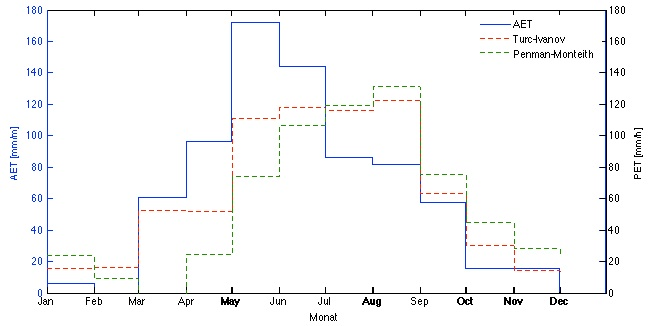
\includegraphics[width=0.8\textwidth]{figures/lys1_aet_pet_m.jpg}
\caption{grafische Darstellung der monatlichen realen Evapotranspiration und monatlichen potentiellen Evapotranspiration nach Penman-Monteith und Turc-Ivanov}
\label{fig:aet_pet_m}
\end{figure}


\subsection{Vergleich Raps und Weizen}
Die Lysimeterdaten zeigen, dass die maximale reale Evapotranspiration des Weizens ein Monat später erreicht wird, als dies bei Raps der Fall ist. Alle übrigen Aussagen können vom Raps auf Weizen übertragen werden. Dies ist in Abbildung\,\ref{fig:aet_m} ersichtlich.

\begin{figure}[H]
{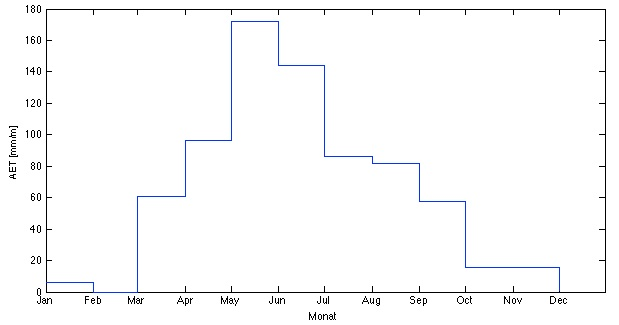
\includegraphics[width=0.49\textwidth]{figures/lys1_aet_m.jpg}} 
{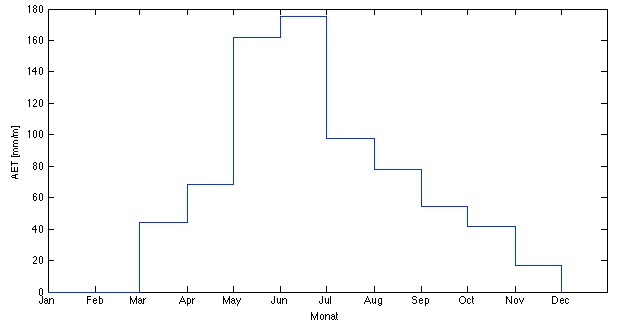
\includegraphics[width=0.49\textwidth]{figures/lys2_aet_m.jpg}} 
\caption{die monatliche reale Evapotranspiration in der linken Abbildung von Raps und in der rechten Abbildung jene von Weizen}
\label{fig:aet_m}
\end{figure} 


\subsection{Sensitivitätsanalyse}
Die Penman-Montheit Methode zeigt gegenüber allen Parametern eine in etwa gleich grosse Sensitivität. Die Methode nach Turc zeigt die grösste Sensitivität gegenüber der relativen Luftfeuchtigkeit und die Lufttemperatur hat den kleinsten Einfluss. Die Methode nach Ivanov reagiert auf beide Parameter Lufttemperatur und relative Luftfeuchtigkeit etwa gleich empfindlich. Die genauen Resultate und die Berechnung sind im Anhang\,\ref{sec:sensitivitaet} ersichtlich.